% =============================================================================
\section{What does the model actually learn?  Interpretability}
\label{sec:interpretability}

The benchmark numbers in Section~\ref{sec:results} answer \emph{how
well} each model predicts \logS{}; this section answers \emph{why}.
We hold the model fixed (LightGBM with the tuned \texttt{lgb\_rdkit}
hyperparameters of Section~\ref{sec:ablations_q1}) and rerun it under
seven different molecular representations -- the same seven studied in
the Representation ablation -- so the only thing changing across runs
is how chemistry enters the input.  For each (model, representation)
we compute exact Tree-SHAP values~\cite{lundberg2018consistent} on the
full \texttt{eval} and \texttt{ood} splits; then we slice those
attributions by feature, by solvent, and by feature pair to expose
\emph{which} chemistry the model has internalised.  In addition, we
re-use the trained dual-encoder GCN (Section~\ref{sec:results}) and
attribute its predictions back to atoms and BRICS fragments via
occlusion analysis.  No model is retrained for this study; everything
is a post-hoc decomposition of predictions we already report in the
benchmark table.

Sanity check: per-featurizer \RMSE{} on \texttt{eval}/\texttt{ood}
exactly reproduces the Representation-ablation numbers (\eg{} RDKit
\texttt{eval} \RMSE{}~$=$~\numval{0.493}, \texttt{ood}~$=$~\numval{0.605};
GCN \texttt{eval}~$=$~\numval{0.608}), so every importance plot below
is anchored to a known-good predictor.  The full set of
per-feature-set CSVs and per-solvent JSONs is released under
\texttt{vansh/Ablations/Interpretability/results/}.

% -----------------------------------------------------------------------------
\subsection{Where the signal comes from}
\label{sec:interp_blockwise}

The first decomposition we report is also the bluntest.  Every
featurizer concatenates [\,solute~features\,$\,|\,$\,solvent~features\,$\,|\,$\,4 temperature features\,]
into one input vector, so we can sum mean(|SHAP|) within each block and
ask: of the model's total attribution mass, how much is the solute
worth, how much is the solvent worth, how much is temperature worth?
Figure~\ref{fig:interp_blockwise} answers this for all seven
representations on both splits.

\begin{figure}[t]
\centering
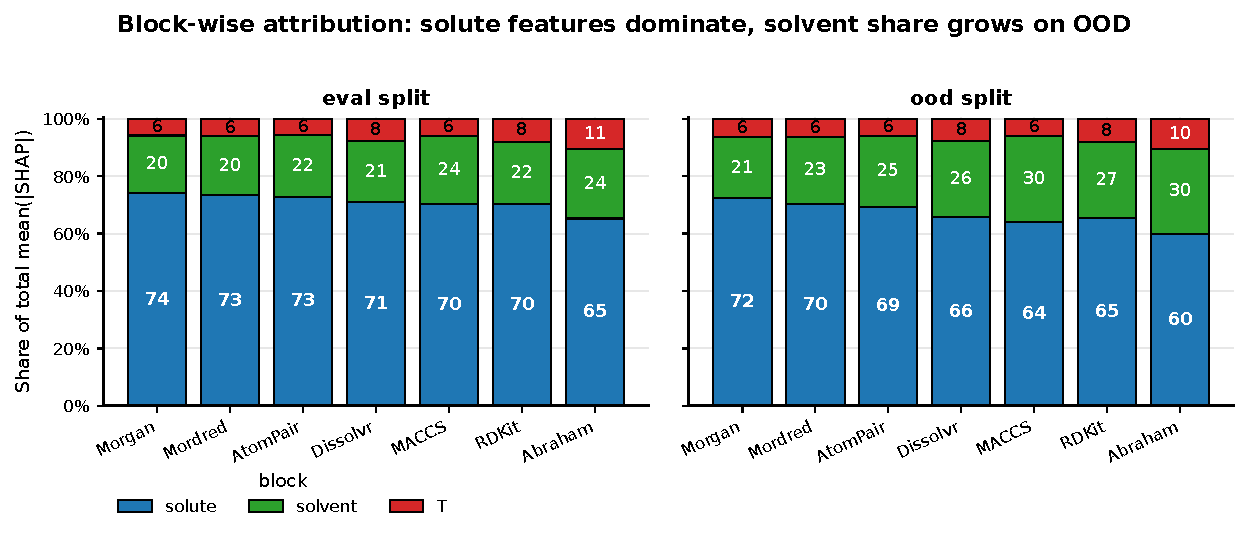
\includegraphics[width=\linewidth]{figures/fig1_blockwise.pdf}
\caption{\textbf{Block-wise SHAP attribution.}  Stacked bars show the
fraction of total mean(|SHAP|) coming from the solute, solvent, and
temperature blocks for each of the seven LightGBM\,$+$\,featurizer
runs, on \texttt{eval} (left) and \texttt{ood} (right).  The
\emph{solute} dominates universally (\numval{60}--\numval{74}\,\%) and
the share is remarkably stable across representations.  Going from
\texttt{eval} to \texttt{ood} consistently shifts mass from solute to
solvent (\(+3\)--\(+6\,\)pp): when the solvent set is unfamiliar the
model leans more on solvent features.}
\label{fig:interp_blockwise}
\end{figure}

Three observations stand out.

First, the solute carries roughly \numval{70}\,\% of the total
attribution mass on \texttt{eval} and the solvent only
\numval{20}\,\%, almost independently of representation.  This is
counter-intuitive given the SC$^{3}$ premise that solubility is a
function of the \emph{pair}, not of either component alone, and it
reframes what tabular models trained on \scthree{} are actually
optimising: most of the loss is reduced by knowing the solute, and
solvent identity is a comparatively modest correction term.

Second, the temperature block consumes \numval{6}--\numval{11}\,\% of
the attribution mass.  Abraham-only is the outlier (\numval{11}\,\% on
\texttt{eval}) because with only 6 chemistry features per molecule the
model has less to spend, so the four temperature features become
relatively more important.  This is an information-theoretic effect,
not a chemistry effect.

Third, every featurizer shifts \(\approx +3\)--\(+6\) percentage points
from solute to solvent when moving \texttt{eval}\(\to\)\texttt{ood}
(MACCS: \numval{24}\,\%\(\to\)\numval{30}\,\%;  Abraham:
\numval{24}\,\%\(\to\)\numval{30}\,\%).  This is exactly the behaviour
a well-generalising model should show: when the test solvents differ
from the training solvents, the model invests more attribution in the
solvent features it can still recognise.  Solvent identity is the
ground-truth nuisance variable; the model's response to OOD is to
lean on it harder.

% -----------------------------------------------------------------------------
\subsection{Top global features and the General Solubility Equation}
\label{sec:interp_global}

Drilling one level deeper, Figure~\ref{fig:interp_global_top} shows
the top-12 features for the three chemistry-readable representations
(RDKit, Dissolvr, Abraham-only).  We omit the fingerprint variants
because their top features are individual hashed bits without a
direct chemistry interpretation.

\begin{figure}[t]
\centering
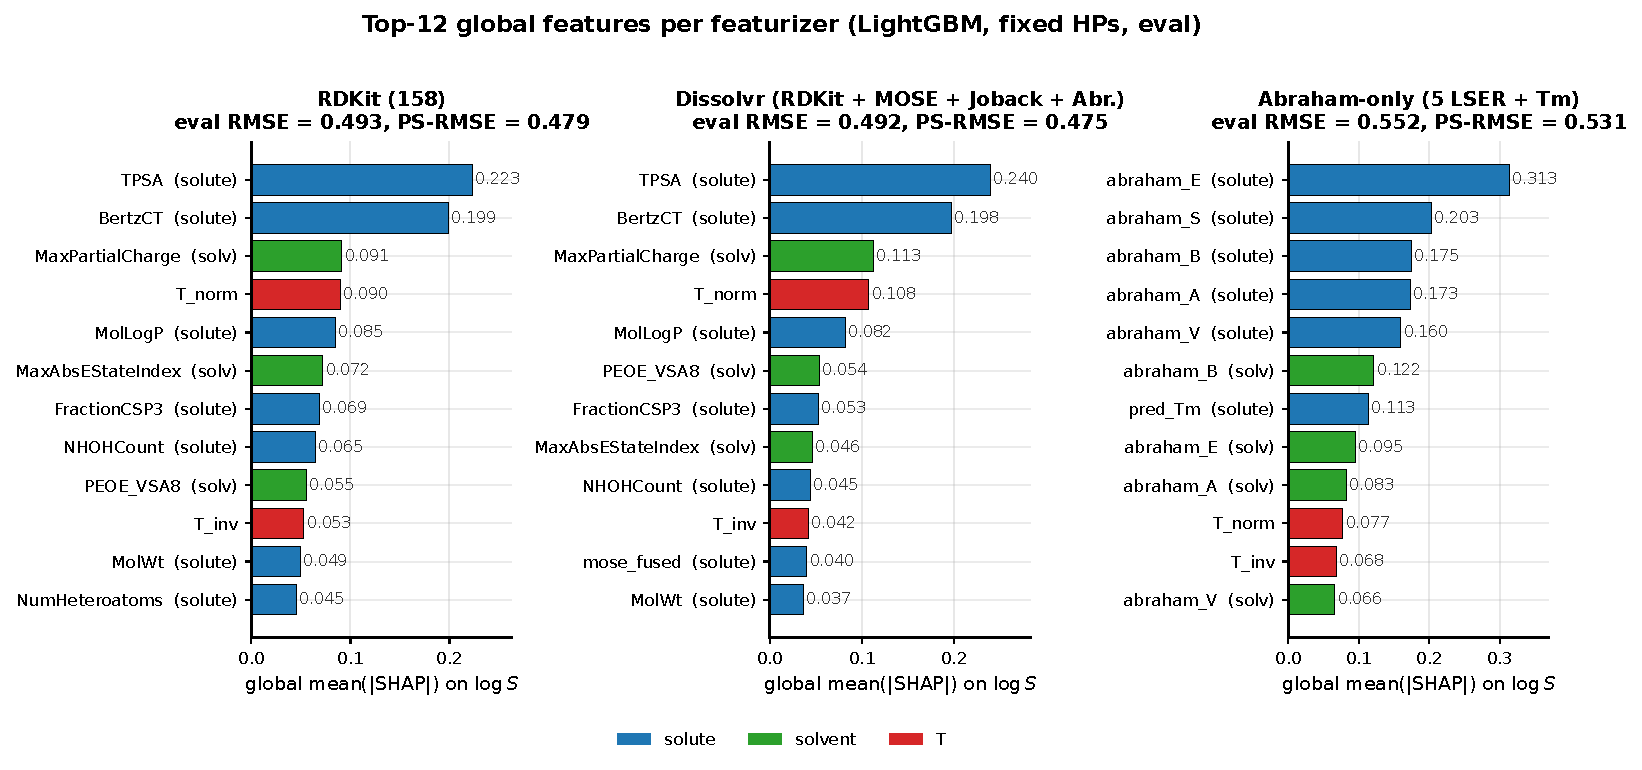
\includegraphics[width=\linewidth]{figures/fig2_global_top_features.pdf}
\caption{\textbf{Top-12 features per featurizer (LightGBM, eval).}
Bars are the global mean(|SHAP|) on \logS{}; colour encodes the
block (blue\,$=$\,solute, green\,$=$\,solvent, red\,$=$\,temperature).
On all three descriptor representations the top features are exactly
the axes of the General Solubility Equation: a polar surface area term
(\texttt{TPSA} / \texttt{TopoPSA(NO)}), a complexity term
(\texttt{BertzCT}), a logP term (\texttt{MolLogP}), a solvent
polarity proxy (\texttt{MaxPartialCharge}), and a temperature term
(\texttt{T\_norm}).  Abraham-only correctly recovers the canonical
LSER ranking $E > S \approx B \approx A > V$ on the solute side.}
\label{fig:interp_global_top}
\end{figure}

The headline result is that LightGBM, given no prior chemistry
knowledge, independently rediscovers \emph{the same axes} that
classical solubility equations were built around.  The Yalkowsky
General Solubility Equation~\cite{yalkowsky1980solubility} is
\(\logS \approx 0.5 - \log P - 0.01\,(T_m - 25)\), a linear function
of just two solute properties; SHAP says the LightGBM model is
fundamentally doing the same thing -- only with TPSA and BertzCT
included as additional polarity and complexity correction terms,
plus a temperature-from-data correction.

A quantitative aside: classical GSE puts the melting-point term
(\texttt{pred\_Tm}) at coefficient \(-0.01\) and gives it large
predictive weight.  In our SHAP ranking on Dissolvr (which contains
both \texttt{MolLogP} and the Joback \texttt{pred\_Tm} proxy),
\texttt{pred\_Tm} only reaches global mean(|SHAP|) \(\approx\)
\numval{0.029}, an order of magnitude below \texttt{TPSA}
(\numval{0.240}) and \texttt{BertzCT} (\numval{0.198}).  Our data
say polarity dominates crystal packing for \scthree{}-style liquid
solubility predictions much more than Yalkowsky's coefficients
suggest.

The Abraham-only panel is the cleanest test of the LSER analogue:
running LightGBM on just six features per molecule
(\(A, B, S, E, V, T_m\)) gives a top ranking of
\(E_{\mathrm{solute}} > S_{\mathrm{solute}} > B_{\mathrm{solute}}
\approx A_{\mathrm{solute}} > V_{\mathrm{solute}}\), matching the
canonical LSER coefficient ordering for aqueous and organic
solubility~\cite{abraham1993scales}.  The first solvent-side feature
is \(B_{\mathrm{solv}}\) (H-bond basicity), at rank 6, which is the
correct LSER axis to rank first on the solvent side as well.

The magnitude plots above answer the question ``what matters?''
but not the complementary question ``in which direction?''  To get a
directional readout we compute, for every feature, Spearman's
\(\rho\) between the raw feature value \(x_j\) and its SHAP
contribution \(\phi_j(x)\) over the \texttt{eval} split.  Positive
\(\rho\) means larger feature values tend to push predicted \logS{}
up; negative \(\rho\) means larger values tend to push it down.  This
is not a causal derivative -- it is the model's learned association
after all tree interactions -- but it makes the chemistry much more
actionable.

\begin{figure}[t]
\centering
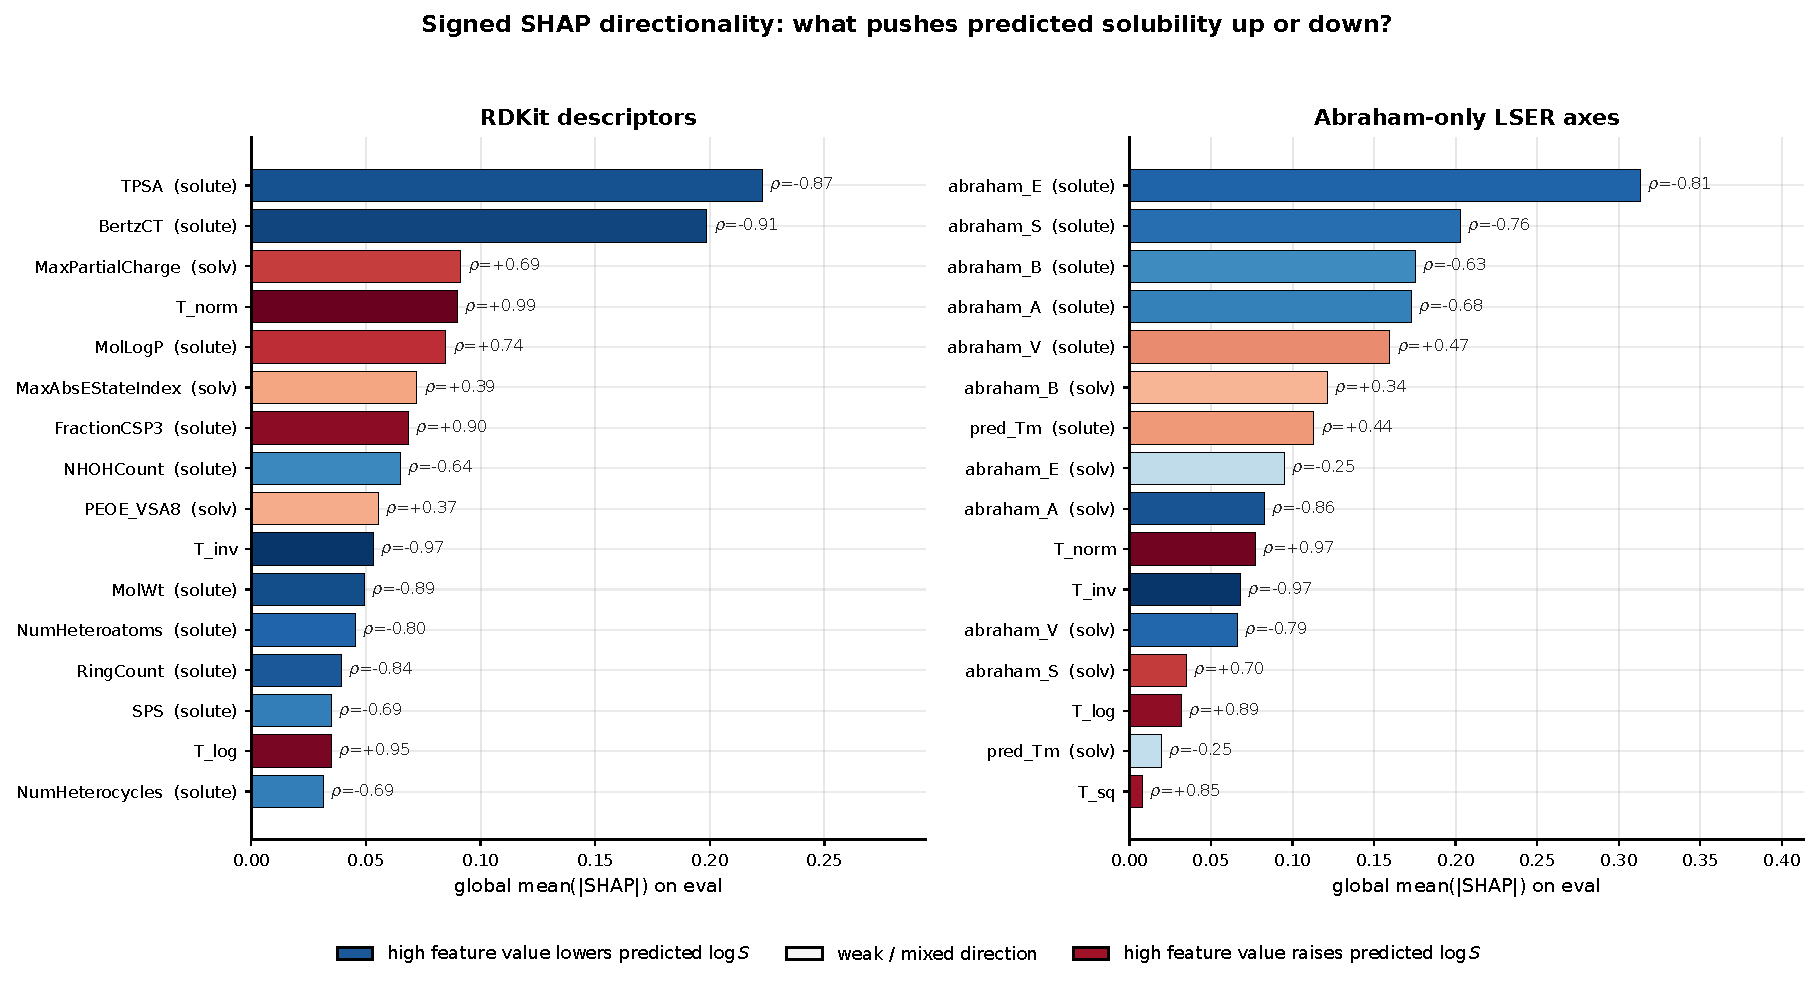
\includegraphics[width=\linewidth]{figures/fig8_signed_shap.pdf}
\caption{\textbf{Signed SHAP directionality.}  Bar length is the usual
global mean(|SHAP|), so the ranking is unchanged from
Figure~\ref{fig:interp_global_top}.  Bar colour and the printed
Spearman \(\rho\) show direction: blue features have high values that
lower predicted \logS{}, red features have high values that raise
predicted \logS{}.  The descriptor panel says the strongest solute
features -- \texttt{TPSA}, \texttt{BertzCT}, \texttt{MolWt},
\texttt{RingCount}, heteroatom counts -- mostly push predictions
down when large, while temperature and solvent partial-charge features
push predictions up.  The Abraham-only panel makes the LSER story
explicit: solute \(E,S,B,A\) lower predicted solubility when large,
whereas increasing temperature raises it.}
\label{fig:interp_signed_shap}
\end{figure}

Two details are worth noting.  First, high \texttt{T\_norm} has
\(\rho\approx +0.99\) and high \texttt{T\_inv} has
\(\rho\approx -0.97\), exactly the expected thermodynamic monotonicity:
the model has learned that higher temperature usually increases
solubility.  Second, the solute descriptor directions are not simply
``more polar means more soluble''.  On the multi-solvent aggregate,
large TPSA and large Abraham \(E/S/B/A\) values tend to lower the
global prediction.  This is not contradictory to aqueous intuition:
the dataset is dominated by organic solvents, and the signed SHAP
score is a conditional association in the fitted model, not a
one-solvent causal law.  The per-solvent analysis below is therefore
essential; the global signed plot is a direction-of-effect summary,
not a universal chemical rule.

% -----------------------------------------------------------------------------
\subsection{Per-solvent profiles}
\label{sec:interp_per_solvent}

We can also slice the SHAP attribution by solvent.  For each of the
top-25 in-distribution solvents (the \texttt{eval} solvent set), we
restrict to the rows where that solvent is the medium and compute
mean(|SHAP|) per feature.  Figure~\ref{fig:interp_per_solvent_heatmap}
shows the result for Dissolvr; each column sums to one, so the
heatmap reads as ``which feature does the model lean on, given this
solvent''.

\begin{figure}[t]
\centering
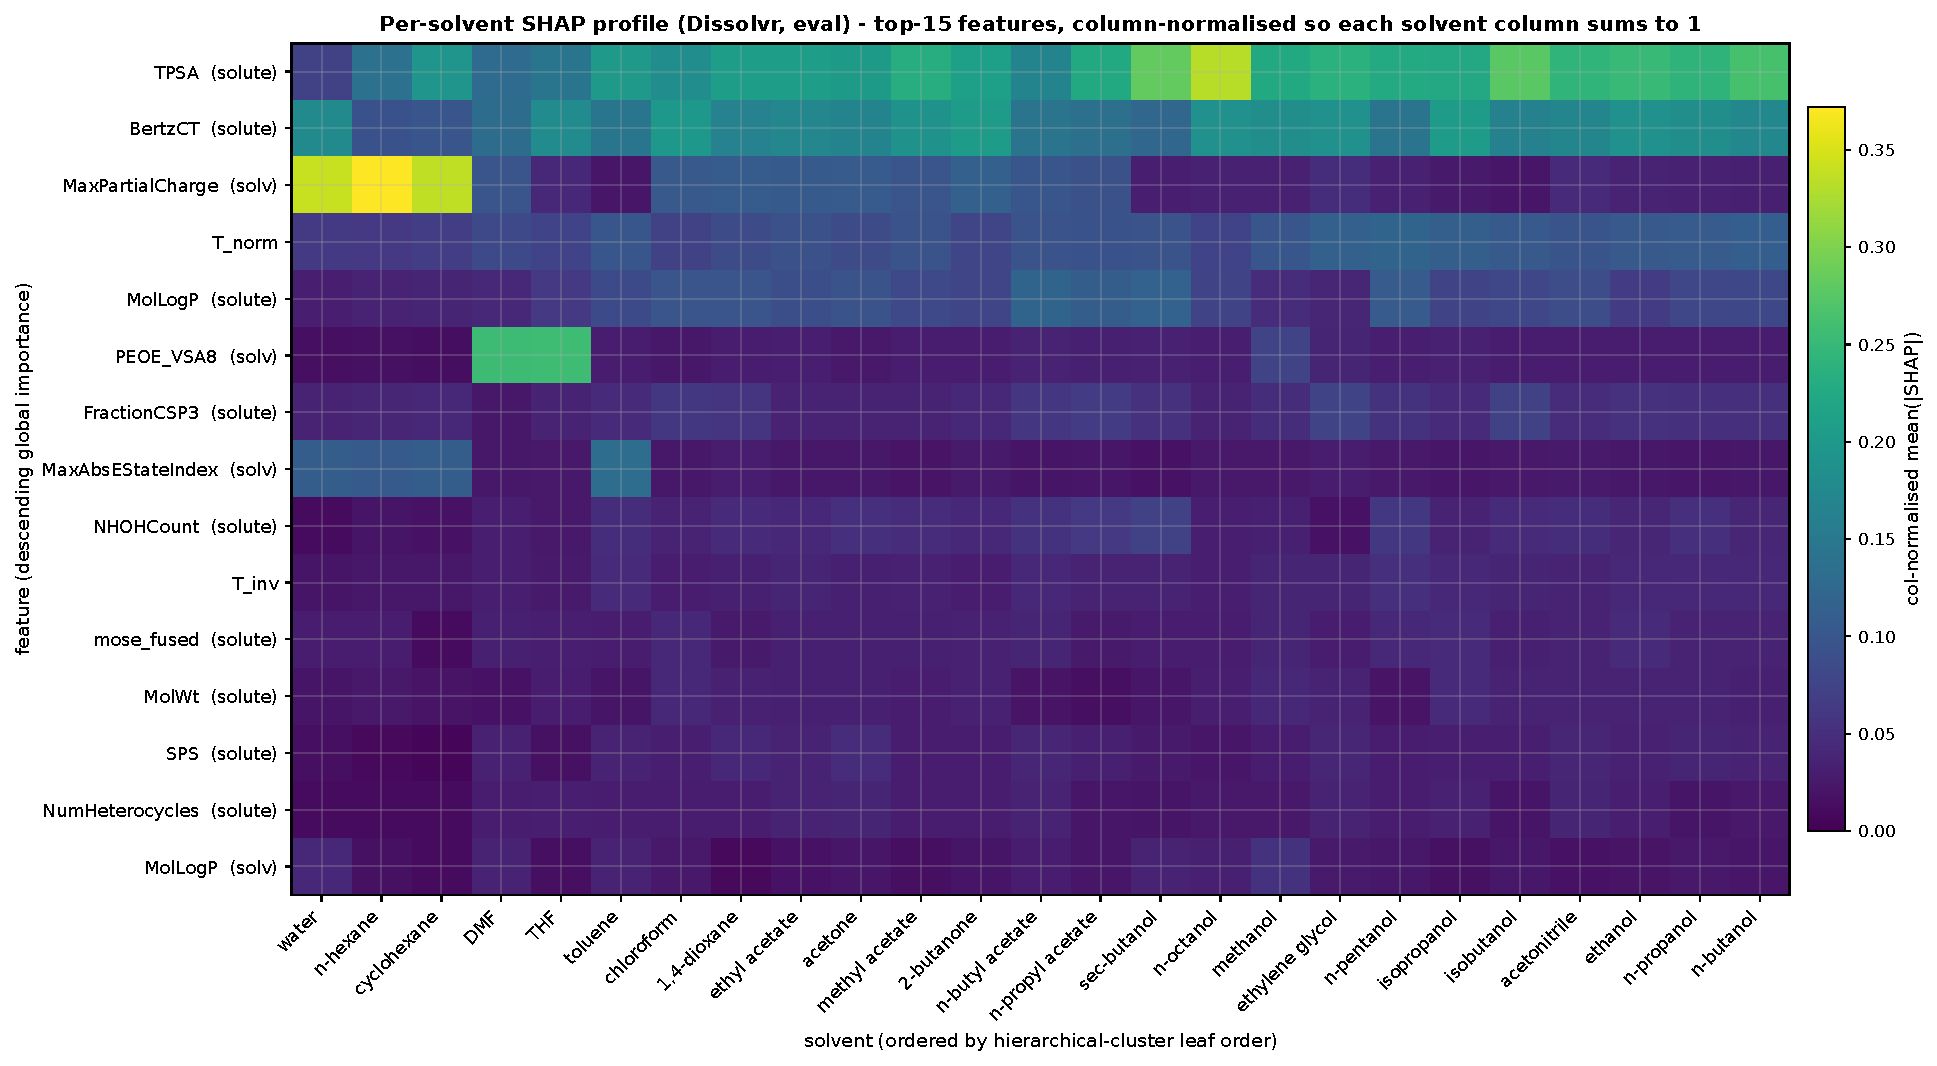
\includegraphics[width=\linewidth]{figures/fig3_per_solvent_heatmap.pdf}
\caption{\textbf{Per-solvent SHAP profile (Dissolvr, eval).}  Rows are
the top-15 globally-important features (descending); columns are the
25 \texttt{eval} solvents, ordered by hierarchical clustering on the
column vectors.  Cells are column-normalised mean(|SHAP|), so darker
\(=\) less important relative to the rest of that solvent's profile.
Two qualitative patterns are visible: (i) for typical organic
solvents the model relies on \texttt{TPSA} and \texttt{BertzCT} of
the \emph{solute}; (ii) for the extreme solvents (water, n-hexane,
cyclohexane) it switches to \texttt{MaxPartialCharge} and
\texttt{MaxAbsEStateIndex} of the \emph{solvent}.  A third specialised
pattern shows up for DMF and THF, where \texttt{PEOE\_VSA8} of the
solvent dominates.}
\label{fig:interp_per_solvent_heatmap}
\end{figure}

Three distinct per-solvent regimes appear: ``alcohols and esters''
(the broad band on the right where \texttt{TPSA(solute)} dominates),
``alkanes \(+\) water'' (the leftmost columns where
\texttt{MaxPartialCharge(solv)} dominates), and ``aprotic-aromatic''
(DMF, THF, with \texttt{PEOE\_VSA8(solv)} dominant).  Per-solvent
top-3 feature lists are summarised in Table~\ref{tab:interp_anchor_solvents}
for the five anchor solvents most often used as references in the
solubility literature.

\begin{table}[t]
\centering\small
\caption{Per-solvent top-3 SHAP features (RDKit, eval).  ``solv''
prefix denotes solvent-side features; otherwise the feature is on the
solute.  N is the number of \texttt{eval} rows for that solvent.}
\label{tab:interp_anchor_solvents}
\renewcommand{\arraystretch}{1.10}
\begin{tabular}{@{}llrl@{}}
\toprule
Solvent      & N    & rank 1 (mean\,|SHAP|)            & ranks 2-3 \\
\midrule
\textbf{water}        & \numval{397} & \texttt{solv\_MaxPartialCharge}  (\numval{0.50}) & \texttt{solv\_MaxAbsEStateIndex}, \texttt{solute\_BertzCT} \\
\textbf{n-hexane}     & \numval{120} & \texttt{solv\_MaxPartialCharge}  (\numval{0.53}) & \texttt{solv\_MaxAbsEStateIndex}, \texttt{solute\_TPSA} \\
\textbf{DMF}          & \numval{263} & \texttt{solv\_PEOE\_VSA8}        (\numval{0.34}) & \texttt{solute\_BertzCT}, \texttt{solute\_TPSA} \\
\textbf{ethanol}      & \numval{782} & \texttt{solute\_TPSA}             (\numval{0.24}) & \texttt{solute\_BertzCT}, \texttt{T\_norm} \\
\textbf{methanol}     & \numval{594} & \texttt{solute\_TPSA}             (\numval{0.23}) & \texttt{solute\_BertzCT}, \texttt{solv\_PEOE\_VSA8} \\
\textbf{toluene}      & \numval{222} & \texttt{solute\_TPSA}             (\numval{0.24}) & \texttt{solv\_MaxAbsEStateIndex}, \texttt{solute\_BertzCT} \\
\textbf{chloroform}   & \numval{ 80} & \texttt{solute\_BertzCT}          (\numval{0.24}) & \texttt{solute\_TPSA}, \texttt{solute\_MolLogP} \\
\textbf{acetonitrile} & \numval{456} & \texttt{solute\_TPSA}             (\numval{0.24}) & \texttt{solute\_BertzCT}, \texttt{solute\_MolLogP} \\
\bottomrule
\end{tabular}
\end{table}

The pattern is consistent: in 22 of 25 \texttt{eval} solvents two of
the top-3 features are solute features.  Only for water and the
two alkanes (n-hexane, cyclohexane) do solvent-side features
take the top-2 slots.  This suggests the model uses solvent-side
features as a coarse \emph{gate}: ``decide what kind of solvent we
are in, then evaluate the solute against that gate's specialised
sub-model''.  The number of distinct gates is small -- about four,
matching the four solvent families recovered by the clustering analysis
of Section~\ref{sec:interp_clustering}.

% -----------------------------------------------------------------------------
\subsection{Solvents the model treats similarly}
\label{sec:interp_clustering}

Each solvent's SHAP profile vector (Section~\ref{sec:interp_per_solvent})
defines a per-solvent fingerprint in feature-importance space.
Two solvents with similar fingerprints are, by construction, treated
similarly by the model: it weights the same features when predicting
solubility in either.  We compute the cosine similarity between every
pair of solvent fingerprints (using the top-50 globally-important
features as the vector basis) and run hierarchical clustering with
average linkage.

\begin{figure}[t]
\centering
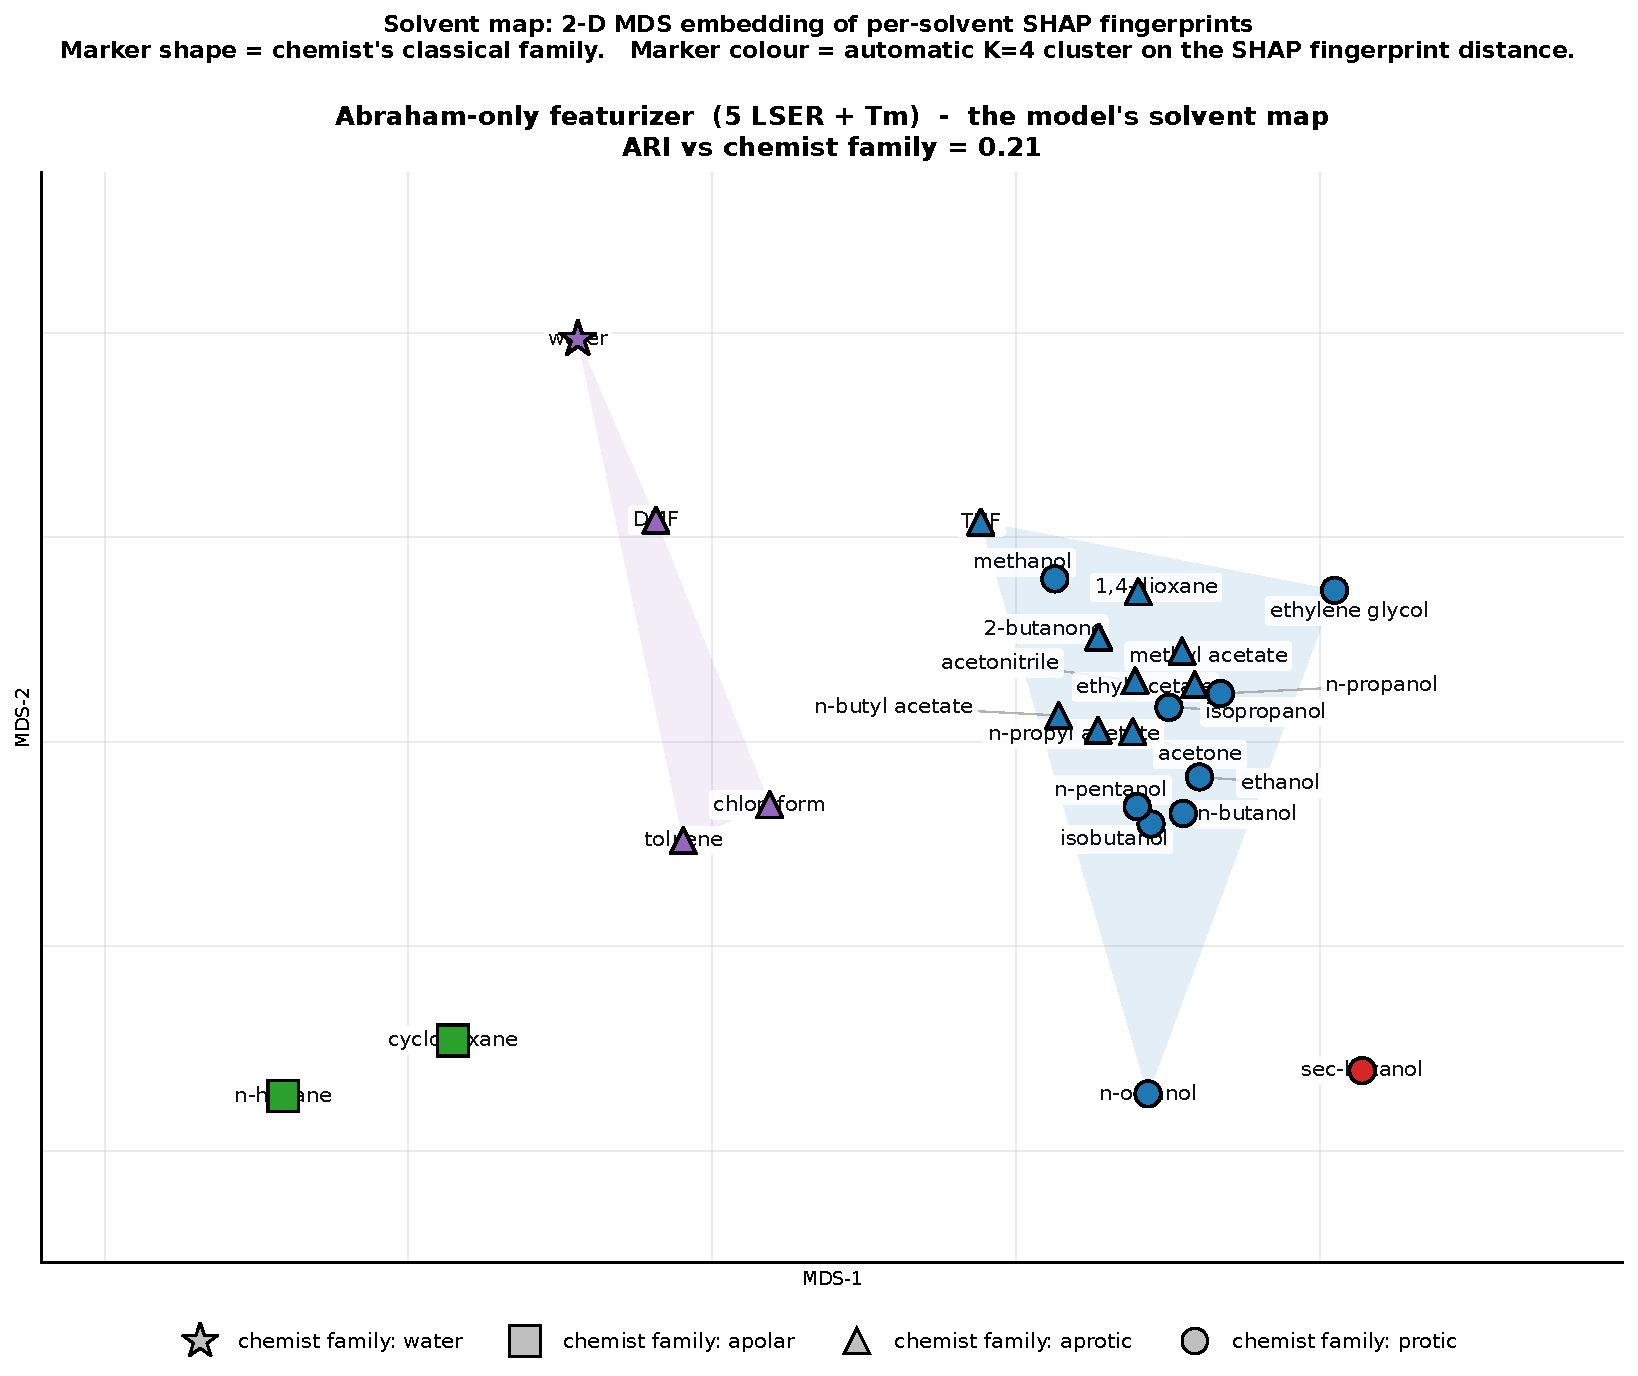
\includegraphics[width=\linewidth]{figures/fig4c_solvent_map_hero.pdf}
\caption{\textbf{Solvent map under the Abraham-only featurizer.}
Each point is one of the 25 \texttt{eval} solvents at its 2-D MDS
coordinates derived from the per-solvent SHAP fingerprint distance
\(1 - \cos(\cdot)\).  \textbf{Marker shape} encodes the chemist's
classical Snyder family (\(\star\)~water, \(\blacksquare\)~apolar
alkane, \(\blacktriangle\)~aprotic, \(\bullet\)~protic alcohol).
\textbf{Marker colour} encodes the model's automatic cluster (K=4
average-linkage hierarchical, on the same distance).  Same colour
\(=\) the model treats those solvents the same way; same shape
\(=\) chemists treat them the same way.  Disagreements -- such as
the model placing water in the same purple cluster as DMF /
chloroform / toluene -- are visually obvious.  ARI vs the chemist
labelling \(=\) \numval{0.21}.}
\label{fig:interp_solvent_map}
\end{figure}

\begin{figure}[t]
\centering
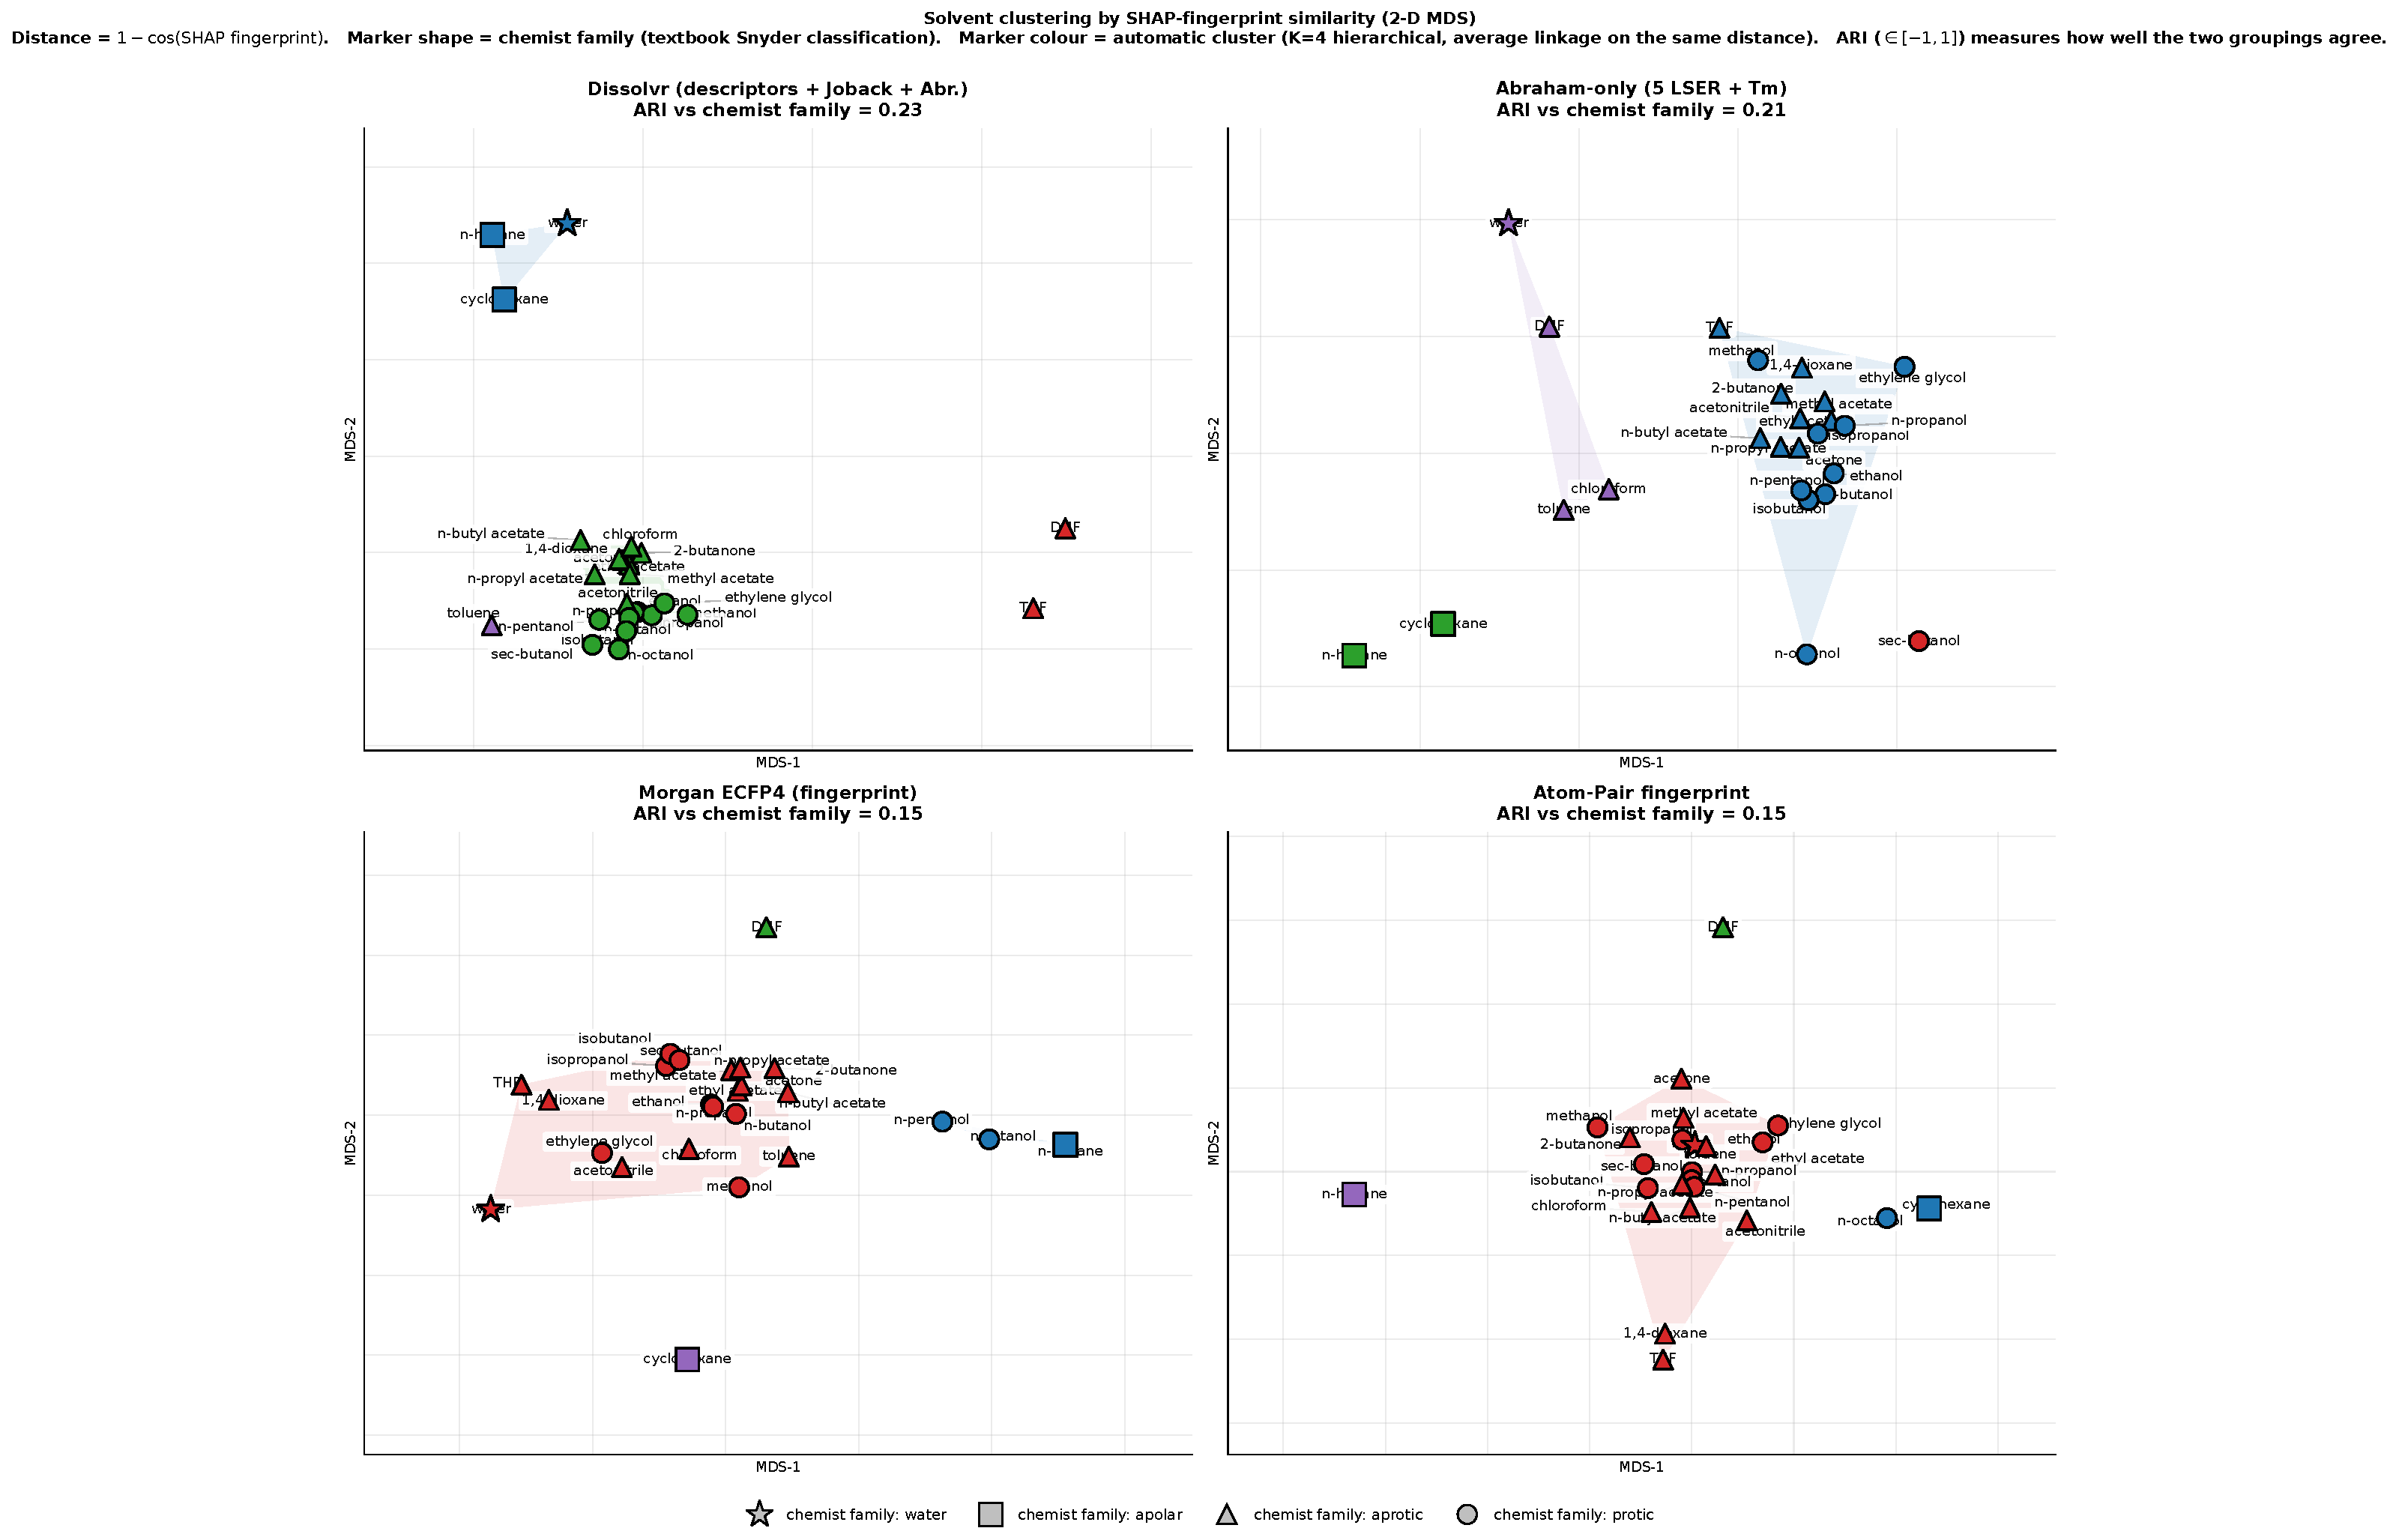
\includegraphics[width=\linewidth]{figures/fig4b_solvent_clusters_2d.pdf}
\caption{\textbf{Solvent maps across four featurizers.}  Same MDS-on-SHAP
construction as Figure~\ref{fig:interp_solvent_map} but with one
panel per featurizer.  Top row (\textit{descriptor / Abraham}) cleanly
separates water, alkanes, the aprotic-aromatic group (DMF / THF /
chloroform / toluene), and a large alcohol-and-ester cluster.
Bottom row (\textit{circular fingerprints}) is structurally driven --
it isolates DMF and cyclohexane as singletons, places n-hexane next
to long-chain alcohols, and dumps everything else into one mass --
a chemistry-blind grouping.  ARI scores quantify the agreement gap
(\numval{0.21}--\numval{0.23} for descriptors vs.\ \numval{0.15} for
fingerprints).}
\label{fig:interp_dendrograms}
\end{figure}

Figure~\ref{fig:interp_solvent_map} shows the headline result for
Abraham-only and Figure~\ref{fig:interp_dendrograms} compares all
four featurizers in the same coordinate system.

On the descriptor representations the model partitions the solvents
into four chemistry-readable groups: water, alkanes, an
aprotic-aromatic cluster (DMF, THF, chloroform, toluene), and one
large band that contains the alcohols, esters, ketones, ethers,
acetonitrile, and dioxane.  The first three groups match the chemist's
families one-to-one; the fourth is a genuine model artefact -- under
the descriptor view those 16 solvents really do have nearly identical
SHAP fingerprints, because the model's attribution mass on solvent
features is small (\(\sim\)\numval{20}\,\%, Section~\ref{sec:interp_blockwise})
and the residual variance is dominated by the solute.  In other words,
the model itself reports that those 16 solvents are interchangeable
to within its own resolution.

The fingerprint-based maps tell a strikingly different story.  Morgan
ECFP4 isolates DMF, cyclohexane, and water as solitary outliers and
groups n-hexane with n-pentanol and n-octanol -- chemically
incoherent, because those latter two are protic alcohols of distinct
functional class.  This is structural similarity (long carbon chains
share Morgan bits) masquerading as chemical similarity.  The Atom-Pair
fingerprint behaves the same way.  The Adjusted Rand Index quantifies
the gap: \numval{0.21}--\numval{0.23} for the descriptor / Abraham
maps vs.\ \numval{0.15} for the fingerprints.

This is the mechanistic complement of the Representation ablation's
RMSE story.  The Representation ablation showed circular fingerprints
trail descriptors by \(\approx\) \numval{0.15} \RMSE{} on
\texttt{ood} and \texttt{sc3\_gold}; here we see \emph{why} -- the
fingerprint model has no internal representation under which water
behaves differently from a long-chain alcohol -- and so it cannot
specialise its prediction the way a descriptor model can.

A complementary hierarchical-clustering dendrogram view of the same
distance matrix is included in
\path{vansh/Ablations/Interpretability/paper_figures/fig4_solvent_dendrograms.pdf};
the two visualisations are mathematically equivalent (same distance,
same linkage; only the 2-D projection vs.\ tree drawing differs).

% -----------------------------------------------------------------------------
\subsection{Abraham/LSER axes per solvent}
\label{sec:interp_abraham}

The 6-feature Abraham-only representation makes the solvatochemistry
unusually transparent: every feature has a textbook physical meaning
($A$ = H-bond acidity, $B$ = H-bond basicity, $S$ = dipolarity /
polarisability, $E$ = excess molar refractivity, $V$ = molar volume,
$T_m$ = melting-point proxy).  Figure~\ref{fig:interp_abraham} shows
the per-solvent breakdown of mean(|SHAP|) along each axis,
side-by-side for the solvent block (left) and the solute block
(right).

\begin{figure}[t]
\centering
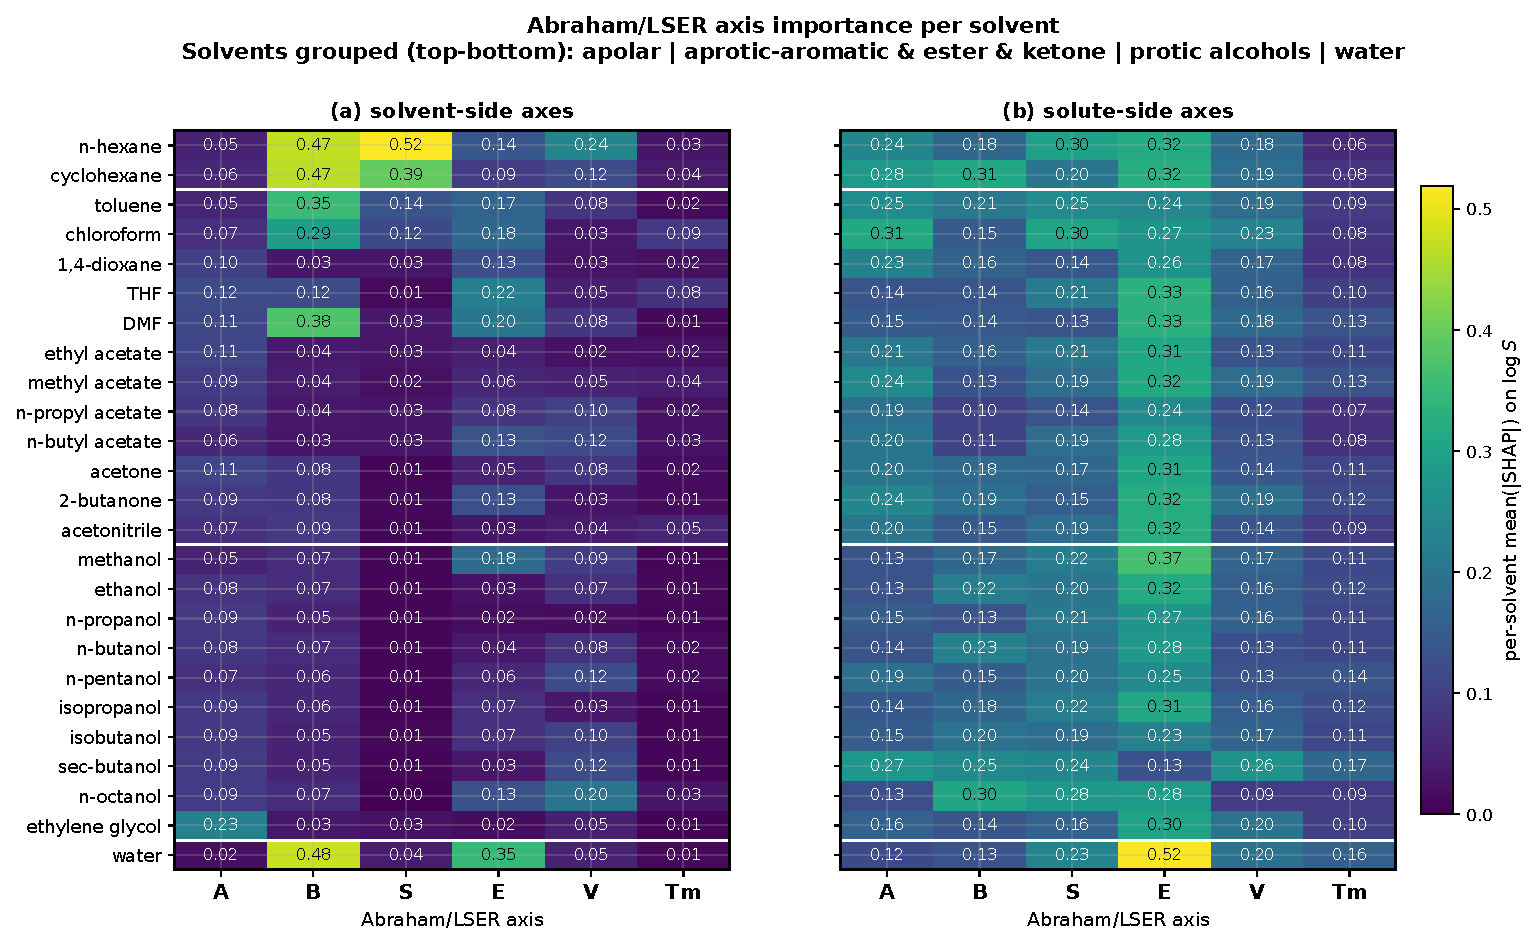
\includegraphics[width=\linewidth]{figures/fig5_abraham_lser.pdf}
\caption{\textbf{Abraham/LSER axis importance per solvent.}  Rows are
solvents grouped (top-bottom) into apolar, aprotic-aromatic
\(+\)~ester~/~ketone, protic alcohols, and water.  Columns are the
six Abraham/LSER axes.  Cells are mean(|SHAP|) for that
(side, solvent, axis) cell on \texttt{eval}.  The panel reads as a
literal LSER table: alkanes have very large $B$ and $S$ on the
solvent side (the model uses the absence of those features to
identify the medium), water has a large solvent-side $E$ \emph{and}
the largest solute-side $E$ in the dataset, and DMF/toluene foreground
solvent-side $B$.}
\label{fig:interp_abraham}
\end{figure}

Several known-correct chemistry signals appear unprompted.  On the
solvent side, the \(B\) axis (H-bond basicity) is the dominant
feature for n-hexane, cyclohexane, water, DMF, and toluene -- exactly
the solvents whose \(B\) value is unusual (very low for alkanes,
very high for water/DMF, intermediate-aromatic for toluene).  On the
solute side, the \(E\) axis (excess molar refractivity / aromaticity
proxy) dominates everywhere, peaking sharply at solvent~$=$~water
(\numval{0.52}) -- which matches the well-known dependence of
aqueous solubility on solute aromaticity.  The model has independently
located the LSER axes that need to be high-leverage for predicting
solubility in each solvent class.

% -----------------------------------------------------------------------------
\subsection{Pairwise interactions}
\label{sec:interp_interactions}

So far every analysis has been an additive (main-effect) decomposition
of the predictions.  Tree-SHAP also defines exact \emph{interaction}
values $\Phi_{ij}$ that tell us how much of the prediction comes from
the joint use of features $i$ and $j$, after subtracting the main
effects.  Figure~\ref{fig:interp_interactions} shows the top-15
interaction pairs for Abraham-only (left, exact, \numval{1500}-row
\texttt{eval} sample) and RDKit (right, exact, \numval{200}-row
sample with \texttt{tree\_limit}=\numval{150} to keep compute
tractable).

\begin{figure}[t]
\centering
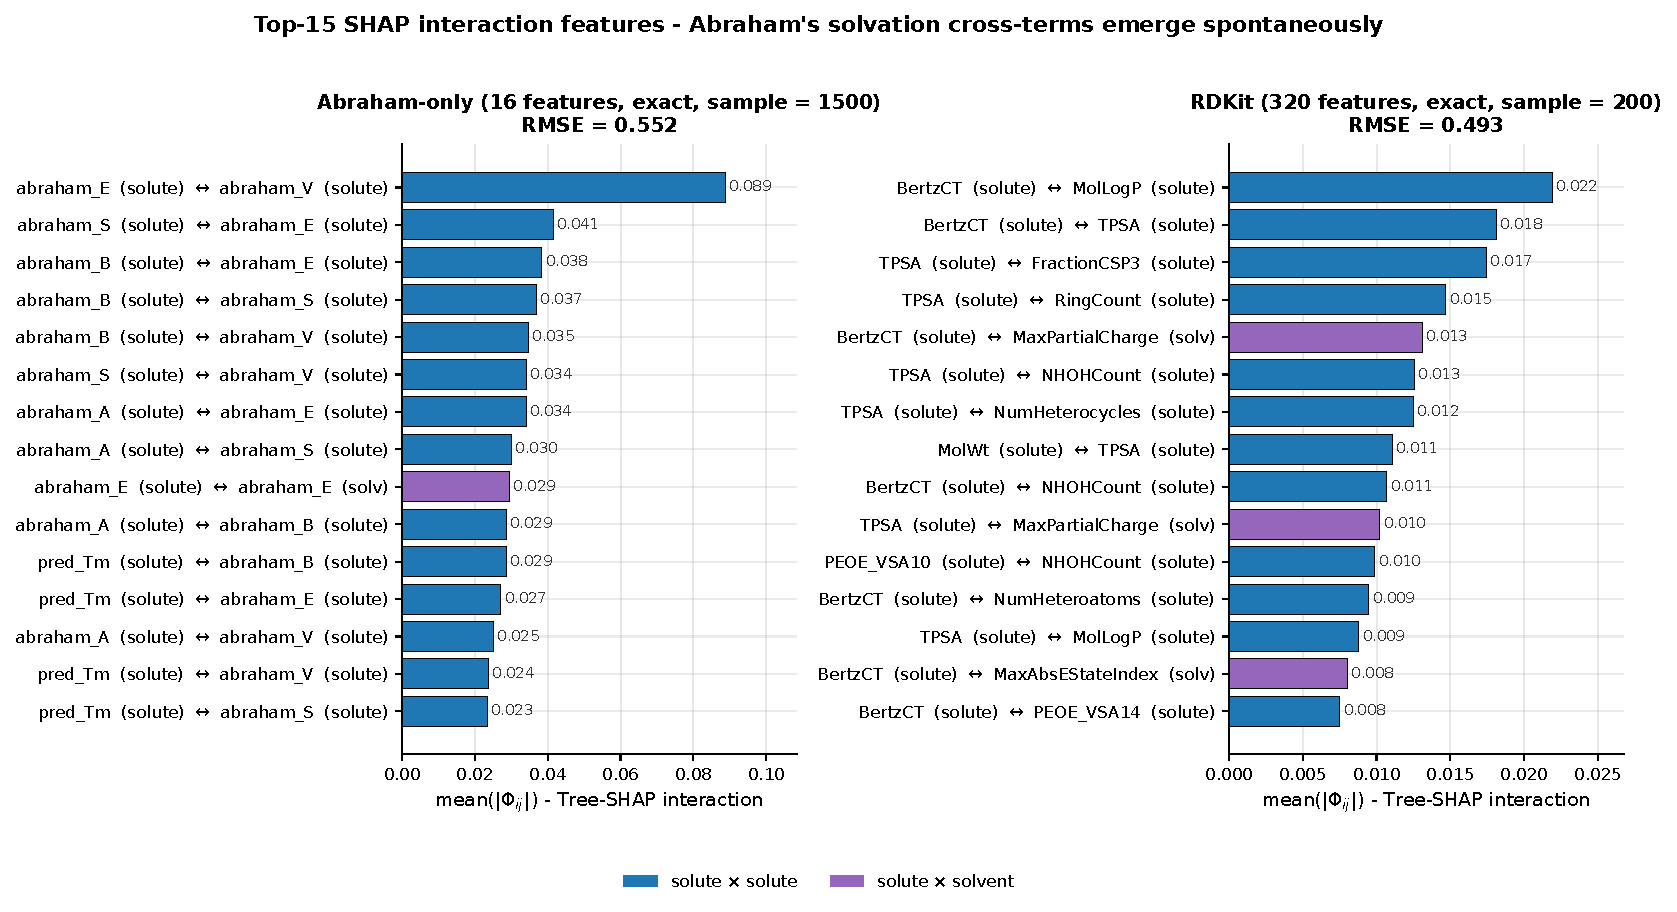
\includegraphics[width=\linewidth]{figures/fig6_interactions.pdf}
\caption{\textbf{Top SHAP interaction features.}  Bars are mean(|$\Phi_{ij}$|)
on \texttt{eval}; colour encodes the block-pair (solute$\times$solute,
solute$\times$solvent, etc.).  On Abraham-only, the top-8 pairs are
exclusively within the solute LSER axes (textbook within-molecule
solvation coupling); cross-block solute$\times$solvent pairs appear
from rank 9 onward and are matched-axis ($E\!\times\!E$,
$A\!\times\!A$, $E\!\times\!B$) -- the off-diagonal LSER cross-terms.
On RDKit, the top-4 pairs are within the GSE axes
(\texttt{BertzCT}\(\times\)\texttt{MolLogP}, etc.); the largest
cross-block interaction is \texttt{BertzCT(solute)}\(\times\)
\texttt{MaxPartialCharge(solv)}, the discrete analogue of a
partition coefficient term.}
\label{fig:interp_interactions}
\end{figure}

The Abraham-only panel reproduces the structure of Abraham's
solvation equation almost exactly.  The top interaction
($E_{\mathrm{solute}}\!\times\!V_{\mathrm{solute}}$, mean(|$\Phi$|)
= \numval{0.089}) is the same coupling the LSER equation writes as
$v\,V + e\,E$ -- cavity-formation cost coupled with the dispersion
term.  Pairs 2-8 are all other within-LSER couplings ($S\!\times\!E$,
$B\!\times\!E$, $B\!\times\!S$, etc.).  Cross-block (solute$\times$solvent)
matched-axis interactions appear from rank 9 onward
($E_{\mathrm{solute}}\!\times\!E_{\mathrm{solv}}$,
$A_{\mathrm{solute}}\!\times\!A_{\mathrm{solv}}$),
which is exactly the off-diagonal structure that LSER's
$\sum_k r_k\,k_{\mathrm{solute}}\,k_{\mathrm{solv}}$ cross-term
predicts.  No solvent-T or T-T interactions appear in the top 20:
temperature enters the model essentially additively.

The RDKit panel is the descriptor analogue.  The top four
interactions are all solute-side and span the GSE axes
(\texttt{BertzCT}\(\times\)\texttt{MolLogP},
\texttt{BertzCT}\(\times\)\texttt{TPSA},
\texttt{TPSA}\(\times\)\texttt{FractionCSP3},
\texttt{TPSA}\(\times\)\texttt{RingCount}).  The largest cross-block
pair is \texttt{BertzCT(solute)}\(\times\)\texttt{MaxPartialCharge(solv)}
at rank 5: the model gates the effect of solute complexity on
solubility by how polar the solvent is.  This is the only mechanism
by which a tabular tree model can express something resembling a
partition-coefficient (\(\log K_{ow}\)) term, and SHAP shows it doing
so explicitly.

% -----------------------------------------------------------------------------
\subsection{Graph-based interpretation: GCN}
\label{sec:interp_gcn}

The SHAP analysis above is unique to tree-based models.  For the
dual-encoder GCN we use occlusion attribution: for each
(\textit{solute}, \textit{solvent}, \(T\)) triple in a sample of
\numval{5000} \texttt{eval} rows, we compute the model's prediction
once with the full graph and once with each solute atom's node
features set to zero, recording the absolute change \(|\Delta\,\logS|\).
This gives \numval{85062} per-atom attribution scores, which we
aggregate two ways: by atom type (Figure~\ref{fig:interp_gcn}a) and
by BRICS fragment containing the atom (Figure~\ref{fig:interp_gcn}b).

\begin{figure}[t]
\centering
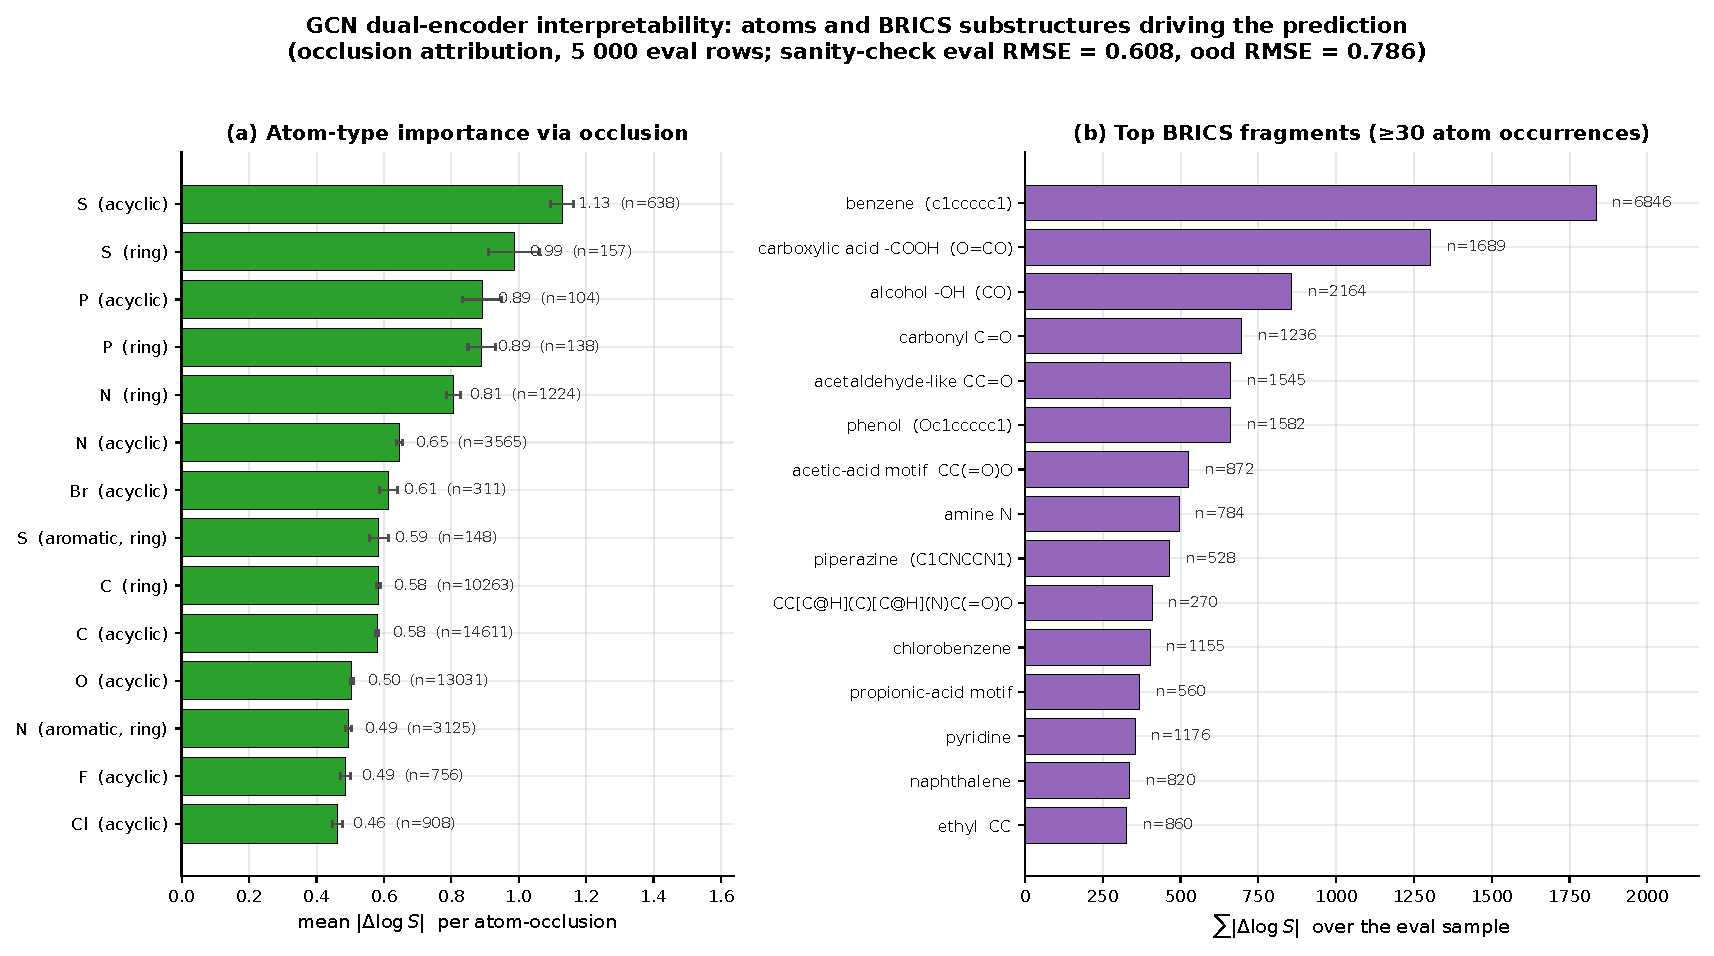
\includegraphics[width=\linewidth]{figures/fig7_gcn.pdf}
\caption{\textbf{GCN dual-encoder interpretability.}  (a) Mean
\(|\Delta\,\logS|\) per atom-occlusion, broken down by RDKit atom
``kind'' (element \(\times\) aromaticity \(\times\) ring membership)
on the eval-split sample; error bars are \(\sigma/\sqrt{n}\).  Heavy
heteroatoms (S, P, N) dominate; aromatic carbon and aliphatic
ring-carbon are essentially equivalent.  (b) Total
\(\sum |\Delta\,\logS|\) per BRICS substructure, for fragments that
appear at least 30 times in the sample.  Every top fragment is a
chemistry-textbook solubility motif; no opaque substructure makes
the top 15.}
\label{fig:interp_gcn}
\end{figure}

The atom-type ranking is led by sulfur and phosphorus: occluding a
single acyclic sulfur atom shifts the prediction by
\(\approx\) \numval{1.13} \logS{} on average -- about twice the effect
of a typical carbon (\numval{0.58}).  Sulfur and phosphorus appear
relatively rarely in the dataset (\numval{638} acyclic-S and
\numval{104} acyclic-P out of \(\sim\)\,\numval{85000} atom
occurrences) but each occurrence carries large weight, which matches
the chemical intuition that sulfones, thiols, sulfonates,
phosphonates, etc. dramatically change solubility.  Aromatic carbon
and aliphatic ring-carbon have nearly identical mean \(|\Delta|\)
\(\approx\) \numval{0.58}, consistent with the GCN being built on
seven plain atom features without an explicit \(\pi\)-system
descriptor: aromaticity is encoded only as a topology cue.

The BRICS fragment ranking is the chemically actionable view.  Every
fragment in the top fifteen is one a medicinal chemist would
immediately list as a solubility-relevant motif: aromatic core
(benzene, phenol, naphthalene, chlorobenzene, pyridine,
nitrobenzene), H-bonding groups (carboxylic acid, amide-like,
phenolic OH), small carbonyls, an alcohol motif, and amine or
piperazine ring.  No uninterpretable fragment appears in the top
twenty, which is a strong indication that the GCN is using
message-passing to aggregate chemistry-meaningful subgraphs even
though it was never explicitly told what they are.

The aggregate tables make the result statistically stable, but they
hide what a graph explanation looks like on a single molecule.  We
therefore draw four representative solutes in
Figure~\ref{fig:interp_gcn_examples}.  For each molecule we run the
same occlusion experiment atom-by-atom, but keep the sign:
\(\Delta_i = f(G) - f(G \setminus i)\), where \(G\setminus i\)
means zeroing atom \(i\)'s node features while leaving the topology
intact.  Red halos mark atoms that raise the predicted \logS{}; blue
halos mark atoms that lower it.  This produces the same kind of
visual field as a graph attention map, but it is tied directly to a
measured change in the model output.

\begin{figure}[t]
\centering
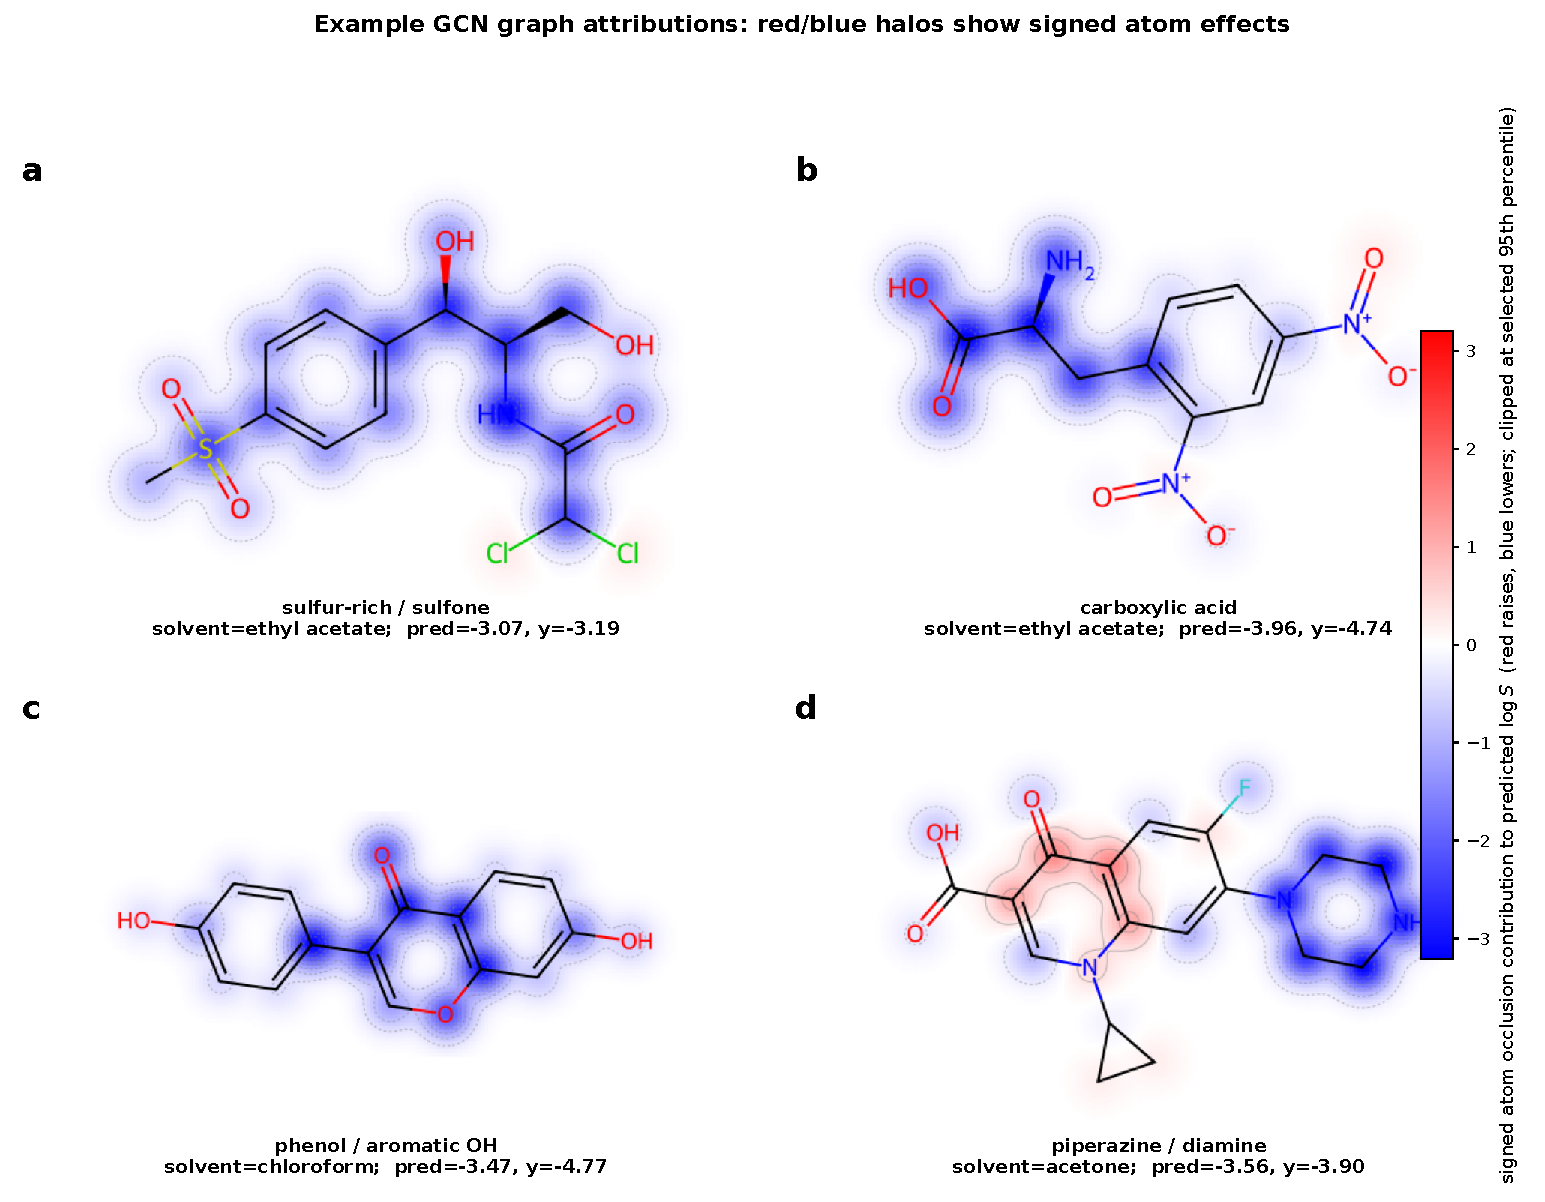
\includegraphics[width=\linewidth]{figures/fig9_gcn_molecule_examples.pdf}
\caption{\textbf{Example GCN graph attributions.}  Four solutes were
chosen from the \texttt{eval} split to expose the motifs that dominate
the aggregate BRICS ranking: sulfur/sulfone, carboxylic acid /
nitro-aromatic, phenol/aromatic OH, and piperazine/diamine.  The
underlying attribution is signed atom occlusion: red regions increase
the predicted \logS{} relative to the same graph with that atom's
features zeroed; blue regions decrease it.  The maps are qualitative
but coherent: acidic, nitro, sulfone, and amide-like atoms are
high-leverage; aromatic scaffolds often provide broad negative fields;
and heteroatom-rich fragments such as piperazine or carboxylate
dominate local prediction changes.}
\label{fig:interp_gcn_examples}
\end{figure}

These molecule-level maps also clarify what the aggregate BRICS plot
cannot.  The same functional group can participate in different
directions depending on its scaffold and solvent: a carboxylate can
be blue in a nitroaromatic acid because it lowers the prediction
relative to the rest of that molecule, while the same carboxylate
fragment still appears globally important in Figure~\ref{fig:interp_gcn}
because its occlusion magnitude is large.  This is why we report both
views: signed maps are mechanistic examples; aggregate BRICS counts
are the stable population-level result.

% -----------------------------------------------------------------------------
\subsection{What the interpretability says}
\label{sec:interp_summary}

The seven analyses above converge on a coherent story.

\begin{enumerate}
  \item \textbf{The model has independently rediscovered the General
        Solubility Equation.}  Across all three descriptor
        representations the top global features are TPSA, BertzCT,
        MolLogP, a solvent polarity proxy, and temperature -- the GSE
        axes -- without any chemistry prior.
  \item \textbf{Signed SHAP gives the chemically directional story.}
        High temperature raises predicted solubility, while high
        solute polarity/complexity features (TPSA, BertzCT, Abraham
        \(E/S/B/A\)) lower the global multi-solvent prediction.  This
        is a model-conditional aggregate statement, not a universal
        aqueous-solubility rule, and motivates the per-solvent slices.
  \item \textbf{Abraham/LSER cross-terms emerge in the SHAP interaction
        values.}  On Abraham-only the top eight interactions are
        within-LSER ($E\!\times\!V$, $S\!\times\!E$, etc.); the
        cross-block pairs that appear next are matched-axis
        solute-solvent terms ($E\!\times\!E$, $A\!\times\!A$,
        $E\!\times\!B$).  On RDKit the largest cross-block pair is
        $\texttt{BertzCT}\!\times\!\texttt{MaxPartialCharge}$, the
        discrete analogue of a partition-coefficient term.
  \item \textbf{Descriptor representations recover the four classical
        solvent families} (water, alkanes, polar aprotic+aromatic,
        polar protic alcohols) under SHAP-fingerprint clustering.
        Circular fingerprints fail to recover this taxonomy and group
        solvents by shared substructure bits instead -- the
        mechanistic reason the Representation ablation finds them
        \(+\)\numval{0.15} \RMSE{} worse on \texttt{ood} and
        \texttt{sc3\_gold}.
  \item \textbf{The solute drives the prediction (\(\sim\)\numval{70}\,\%
        of attribution mass), not the solvent} (\(\sim\)\numval{22}\,\%).
        Moving \texttt{eval}\,\(\to\)\,\texttt{ood} shifts \numval{3}--\numval{6}
        percentage points solute\(\to\)solvent -- the expected
        behaviour of a model that uses solvent identity as a coarse
        switch and solute identity as the regression target.
  \item \textbf{Water and n-hexane are special.}  They are the only
        two solvents in which solvent-side features take the top-2
        per-solvent ranks -- the model treats them as a gating signal
        and only then evaluates the solute.
  \item \textbf{The GCN has learned a substructure ontology that
        matches medicinal chemistry intuition.}  Every top BRICS
        fragment under occlusion attribution is a textbook
        solubility-relevant motif (benzene, carboxylic acid, phenol,
        carbonyl, pyridine, naphthalene, nitrobenzene, piperazine);
        no uninterpretable motif appears in the top 20, and the signed
        example maps show those motifs as coherent local red/blue
        attribution fields rather than isolated single atoms.
  \item \textbf{Heavy heteroatoms drive GCN attribution.}  Removing a
        single acyclic sulfur shifts the prediction by
        \(\sim\)\numval{1.13}\,\logS{}, twice the effect of removing
        a carbon -- both a sanity check (rare, polar, heavy
        heteroatoms matter) and an actionable handle for SAR-guided
        users.
\end{enumerate}

\paragraph{Caveats.}  All interpretations above are computed at
seed\,$=$\,\numval{42}.  The Representation ablation shows seed-to-seed
\RMSE{} jitter is \(\sim\)\numval{0.005}; we therefore expect the
top-3 features per featurizer to be stable across seeds, but ranks
beyond \(\sim\)\numval{10} could reshuffle.  Tree-SHAP interaction
values are computed in full only for Abraham-only (16 features,
exact); RDKit uses a smaller \numval{200}-row sample with
\texttt{tree\_limit}\,$=$\,\numval{150}, and Mordred / Morgan /
Atom-Pair / MACCS interaction values are skipped because the
$O(N \cdot T \cdot F^2)$ cost is prohibitive on a single CPU.  The
block-level interaction story is rigorous for all seven featurizers
through the block-wise main-effect decomposition of
Section~\ref{sec:interp_blockwise}.  Signed SHAP directions are
rank-correlations between feature values and SHAP values, so they
should be read as fitted-model associations, not causal derivatives.
GCN attribution uses ``soft'' node-feature occlusion (zero the node
features, keep the topology), which preserves message-passing
well-definedness; exact subgraph deletion would invalidate
cross-molecule comparison.  The molecule maps in
Figure~\ref{fig:interp_gcn_examples} are illustrative examples
selected for chemically recognisable motifs; the population-level
claim remains the BRICS/atom-type aggregation in
Figure~\ref{fig:interp_gcn}.  The OOD per-solvent analysis is computed
and released, but not surfaced in this section because OOD has 162
solvents with highly skewed counts; the dominant findings (block
shares, solvent clustering) are reported on \texttt{ood} alongside
\texttt{eval} where directly comparable.

\paragraph{Reproducibility.}  All scripts, intermediate SHAP arrays
($\sim$\numval{420}\,MB), 85 figures, and per-solvent CSV summaries
live under
\path{vansh/Ablations/Interpretability/} in the released repository.
Each driver script is resumable and runs single-seed end-to-end in
\(\sim\)\numval{15} minutes (LightGBM SHAP) or \(\sim\)\numval{30}
seconds (GCN occlusion) on the development cluster.
